%% Sample chapter file, for use in a thesis.
%% Don't forget to put the \chapter{...} header onto each file.

\chapter{Description of the work undertaken}
	\section{Discover}
	
During the discovery phase of the project the objective was to become familiar with the CEC environment, i.e. find out what tools are available and how they are being used and gather information about how to best contribute to the organisation. This was to be done while staying as open as possible, allowing any influences or ideas.

At the beginning of the project I had no knowledge about the operations within the Council or which departments would be involved. Some of the questions I wanted to answer included:
\begin{itemize}
\item Are there any activities in the Council similar to the scope of the project (or were there any in the past)?
\item Who would benefit from it and how to give those stakeholders an opportunity to be involved?
\item What questions (in terms of "channel shift") are not answered in the Council?
At what level of abstraction should the analysis be conducted?
\item What IT systems/tools can be used in the project?
\item Who has the necessary understanding of the infrastructure and activities on the architectural level?
\item What else do I not know?
\end{itemize}

		\subsection{Meetings at the Council}
		
Initially the contact person from the Council was Sally Kerr. In response to my questions she arranged a meeting with an enterprise architect Neil Dumbleton. The purpose of the meeting was to give me an opportunity to ask questions regarding organisational structure as well as context of the project.

As it turned out, it was a first meeting in a series. There was no formalised documentation or central place with knowledge about on-going projects that was made available to me. As a result, personal meetings were the only way to understand activity in the Council. Moreover, it was only thanks to good will of many employees at the City of Edinburgh Council that this was possible.

The diagram below shows all the people who I interacted with during the entire project. Connections between different actors represent how I got to know them. Circles with coloured backgrounds highlight people who I spoke with in this phase. Orange colour marks people related with University of Edinburgh, blue is for CEC employees. Level of a circle does not reflect a position in the Council's structure - it is used solely for increasing legibility of the diagram.

\begin{center}
  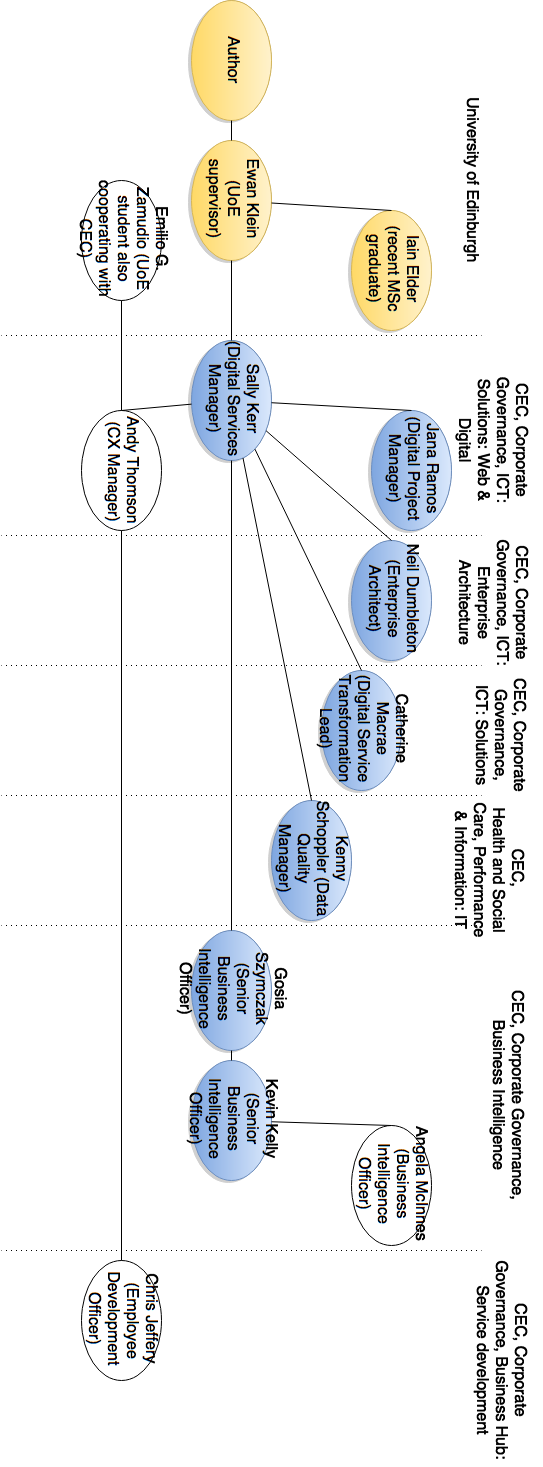
\includegraphics[height=0.95\textheight]{Discovery_phase_people.png}
  \captionof{figure}{CEC employees involved in the project.}
  \label{normal_case}
\end{center}


From these meetings and discussions I gained an initial understanding of the situation at CEC. There was a big effort within the Council aiming at transforming the way services are being delivered and "Channel Shift" was a part of it. The outsourced ICT services in the Council were delivered by British Telecom starting from 2001 and the contract was set to end in 2016. In order to find a new service provider under revised conditions, a public tender was being held during the writing of this thesis. It considered "Channel Shift" as one of the significant enhancements of the Council's operations. Final report suggesting the best bidder was submitted by the Finance and Resources Committee on third of August 2015 \citep{FinanceandResourcesCommittee2016}.

In summer 2014 a new CRM system was introduced called Oracle RightNow. It was replacing the old system called Capture. The deployment was part of the transformation. The system was used to capture information about all interactions with citizens and in some cases it meant that entries did not have all the values specified (due to the nature of an inquiry). The incompleteness of entries did not make them useless as they could still inform about things like level of use. The data captured has not been analysed from the angle described in this project (socio-economic insights) and it was confirmed that such analysis would be useful for the Council.

The transformation within the Council was also trying to centralise Business Intelligence capabilities. The BI department had a number of responsibilities and systems. One of those systems was called IBM Cognos. It was fully operational and a number of reports were generated and delivered to other stakeholders. However, the scale of deployment was still unclear and many departments were still figuring out the role the system would play in their operations. Many services required more digitisation and given the strategy, they could potentially use Cognos in the process. CRM data was an example of a dataset that was promising in providing valuable business insights.

Considering the above, the project would develop a piece of work that would increase know-how within the Council (in terms of using data analysis for designing services and interfaces), provide a "case study" and directly deliver business value to the organisation. The tools and datasets that could be used are described in the following sections.

		\subsection{CRM data}
		
The new system used at the Council was called RightNow and was provided by Oracle. It was a cloud service and the data in the system was available to CEC employees after registration (with staff number) and installation of the interface. The database consisted of a number of tables, e.g. "Answers" which was a "knowledge base for consultants". The table used in the project was "Incidents" and it contained information about transactions initiated by citizens (issues reported by them through all channels). This choice was dictated by the scope of the project - de facto by preferences of the clients who were interested in better understanding of the usage patterns of citizens.

Unique Property Reference Number (UPRN) is a number uniquely identifying a household in Edinburgh and thus a person (or a family). The incidents table had a column named UPRN which provided information about who reported the issue. The Mosaic personas (introduced in the next section) were also using UPRN making it possible to link the two datasets. The table had dozens of columns containing information about things like channel used to report the issue, postcode where it was reported, date, Service Level Agreement (SLA).

The incidents table selected for this project (which is a part of the CRM database) apart from storing detailed information on issues reported by citizens provides means for tracking activity across different channels. Some enquires are just general questions and as a result, many entries do not have all values filled in. This enriches the dataset giving a fuller picture of what is happening, i.e. keeping a trace of all enquires.		
		
		\subsection{Mosaic UK Consumer and Demographic data}
		
Mosaic is a dataset created by Experian - credit reference agency. It provides insights about lifestyles and preferences of people across the United Kingdom. It identifies 14 social groups and a total of 57 types within those groups. It was built using more than 450 data variables and the sources include, but are not limited to \citep{Experian2014}:	

\begin{itemize}
\item Census
\item Open Data
\item OFCOM Broadband speeds
\item Higher Education Statistics Authority (HESA)
\item Electoral Roll
\item Council Tax property valuations
\item YouGov's survey of consumers and their financial behaviour
\item British Crime Survey
\end{itemize}

It is highly detailed (e.g. food a person buys based on information from retailers) and granular (every household). It can be used as a numerical dataset (Cognos package) or a descriptive interpretation (Segmentation portal).

Some of the information about a household available in Mosaic includes:

\begin{itemize}
\item Age of members of the household
\item Income
\item Spending structure
\item Property type
\item Contact channel preference
\item Education
\item Access to technology
\end{itemize}
	
For example, selected characteristics of group D, referred to as "Rural Reality", include: rural locations, village and outlying houses, agricultural employment, affordable value homes, slow Internet speeds. People in this group are aged 66+, they have income of \pounds 20k - \pounds 29k, they live alone (or in "pseudo families") and compared to the rest of the population are less likely to have children. They live in bungalows, named buildings or semidetached households in majority owned by them. Comparing to the rest of the population in the UK, they are half as likely to prefer being contacted via  mobile call (versus a landline). The majority of them use "pay as you go" tariffs with a mobile bill of \pounds 10 or less, they read regional papers and are very likely to do groceries in Co-op and very unlikely to buy in Waitrose. Much bigger part of this group (compared to other groups in the UK) is likely to use e-mail monthly and not listen to music using mobile technologies. 

\begin{center}
  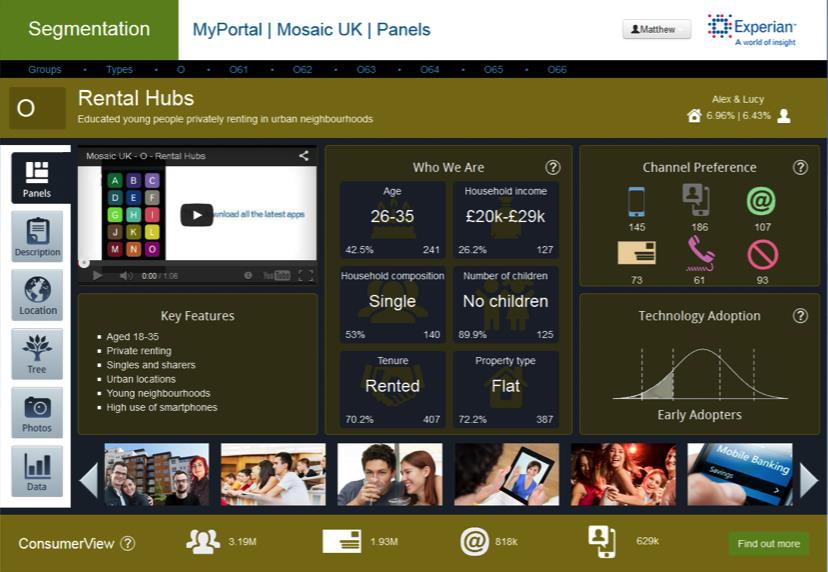
\includegraphics[width=\textwidth]{mosaic_segmentation_portal.jpg}
  \captionof{figure}{Segmentation portal visualising Mosaic data \citep{Experian2014}.}
  \label{normal_case}
\end{center}


		\subsection{IBM Cognos}
		
			\subsubsection{Introduction}
			
Addressing the need of businesses for software that helps to achieve a competitive advantage, IBM has a rich portfolio of analytics products. These include solutions in areas of predictive analytics, risk analytics, prescriptive analytics, enterprise performance management and business intelligence \citep{IBM2015b}. The majority of IBM products in BI belong to the Cognos family and include very specialized applications like "Cognos Supply Chain Performance Procurement Analytics" as well as general purpose tools like "Cognos Business Intelligence".

The solution used at CEC is IBM Cognos Business Intelligence 10.2.1 and it is a set of tools that significantly eases processes such as importing data from different formats (e.g. csv, xml, xlsx), combining relational and multidimensional data, generating reports (real time reports, drag-and-drop GUI, database queries in SQL and OLAP), scheduling and redistributing reports, publishing reports on multiple platforms and many more. Tools available at the CEC include: Report Studio, Query Studio, Analysis Studio.

The same results can be achieved using different tools, but some of them are better fitted for a specific purpose. Report Studio was designed with reports creation in mind, while Query Studio was optimized for creating and editing complex database queries. CEC has two types of instances of IBM Cognos – production and development machines, accessible under different URLs.

IBM Cognos BI is an enterprise class SOA platform \citep{browne2010ibm}. Its n-tiered architecture is made up of:
\begin{itemize}
\item The web tier – provides user sessions connectivity to applications
\item The application tier – load balancing and processing of requests, managing storage of customer application data
\item The data tier
\end{itemize}


\begin{center}
  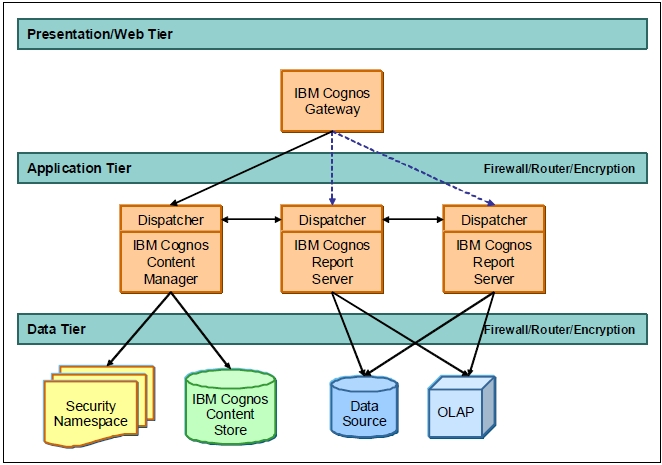
\includegraphics[width=\textwidth]{cognos_architecture.jpg}
  \captionof{figure}{IBM Cognos BI architecture \citep{browne2010ibm}}
  \label{normal_case}
\end{center}


The platform operates by using different services which are run at those three levels \citep{Browne2010}, for example:
\begin{itemize}
\item Agent service – responsible for running agents, "determines which tasks to execute and forwards those tasks to the monitor service for execution"
\item Monitor service – handles requests which will be run in the background including background tasks, reports scheduled to be run and e-mailed, jobs
\item Query service – "manages Dynamic Query Mode requests and returns the results to the requesting batch"
\end{itemize}
		
			
			\subsubsection{Working with IBM Cognos BI}
			
IBM Cognos can be accessed using either a web interface called IBM Cognos Connection or a Windows application. For the purpose of this project only the web interface was used.

\begin{center}
  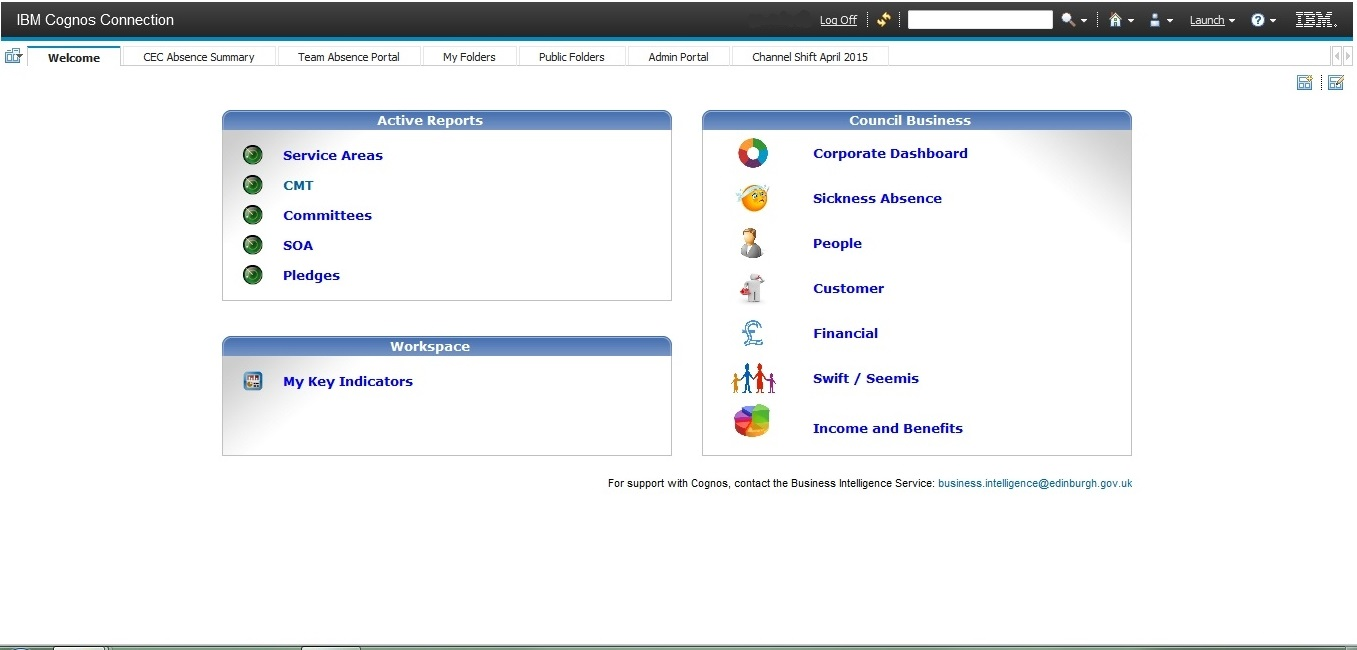
\includegraphics[width=\textwidth]{pre work/1st day Cognos - processed/welcome page of web interface of Cognos.jpg}
  \captionof{figure}{Welcome page of IBM Cognos Connection 10.2.1 (web interface to the entire package)}
  \label{normal_case}
\end{center}


From this welcome page you can start applications available within your license, e.g. Report Studio. The first step after starting Report Studio is selection of the data package that will be used.


After selecting the data package, one can either open an existing report or start creating a new one. In the latter case, a number of templates are available.


The following figure shows Report Studio with a blank report and Mosaic data loaded.


Graphic User Interface (GUI) makes the entire process quick and easy, but it is used to set the general structure of the report. The specifics of the report, e.g. how to filter data, have to implemented using queries.

Example of a single SQL query (filter):
\begin{lstlisting}
if ([No of interactions with CEC] > 3) then ( 'above 3') else ('up to 3')
\end{lstlisting}
Example of a counter:
\begin{lstlisting}
count(rows for [MW].[MW].[Date Created], [MW].[MW].[UPRN], [MW].[MW].[Subject])
\end{lstlisting}
Example of the SQL query used to generate an entire report (the entire report can be exported to an XML format as well):
\begin{lstlisting}
select 
       MW."Creation Source"  as  Creation_Source,
       MW."Group"  as  Group2,
       MW."Date Created"  as  Date_Created,
       MW."Reference #"  as  Reference__,
       MW.Subject  as  Subject,
       MW."Product Hierarchy"  as  Product_Hierarchy,
       MW.UPRN  as  UPRN,
       XCOUNT(MW."Reference #"  at MW.UPRN,MW."Reference #"  for MW.UPRN )  as  No_of_interactions_with_CEC,
       D_MosaicGroupType.GroupTypeCode  as  Group_Type_Code
 from 
       MW...MW MW,
       Mosaic.MosaicExport.dbo.D_MosaicGroupType D_MosaicGroupType,
       Mosaic.MosaicExport.dbo.F_MosaicAddresses F_MosaicAddresses
 where 
       (MW.UPRN = F_MosaicAddresses.Uprn) and 
       (D_MosaicGroupType.GroupTypeId = F_MosaicAddresses.MosaicGroupTypeId)
 group by 
       MW."Creation Source",
       MW."Group",
       MW."Date Created",
       MW."Reference #",
       MW.Subject,
       MW."Product Hierarchy",
       MW.UPRN,
       D_MosaicGroupType.GroupTypeCode
 filter 
       (XCOUNT(MW."Reference #"  at MW.UPRN,MW."Reference #"  for MW.UPRN ) > 3)
 order by 
       Date_Created asc
\end{lstlisting}

	\section{Define}
	
After the discovery phase an understanding of the specifics of the project within the Council has been achieved. The goal of the next phase was to narrow down the scope, find specific questions to be answered and make a decision about tools that would be used. Prototypes were created (simple reports) to prove the capabilities of the system. This phase ended with clear objectives and a general idea of technical aspects of implementing them.	
	
		\subsection{Preliminary work}
		
			\subsubsection{Meetings at the Council}
			
The diagram below shows all people I interacted with in the entire project with those I spoke with in this phase highlighted by coloured background. Orange background being for University related people and blue for people working for CEC.


\begin{center}
  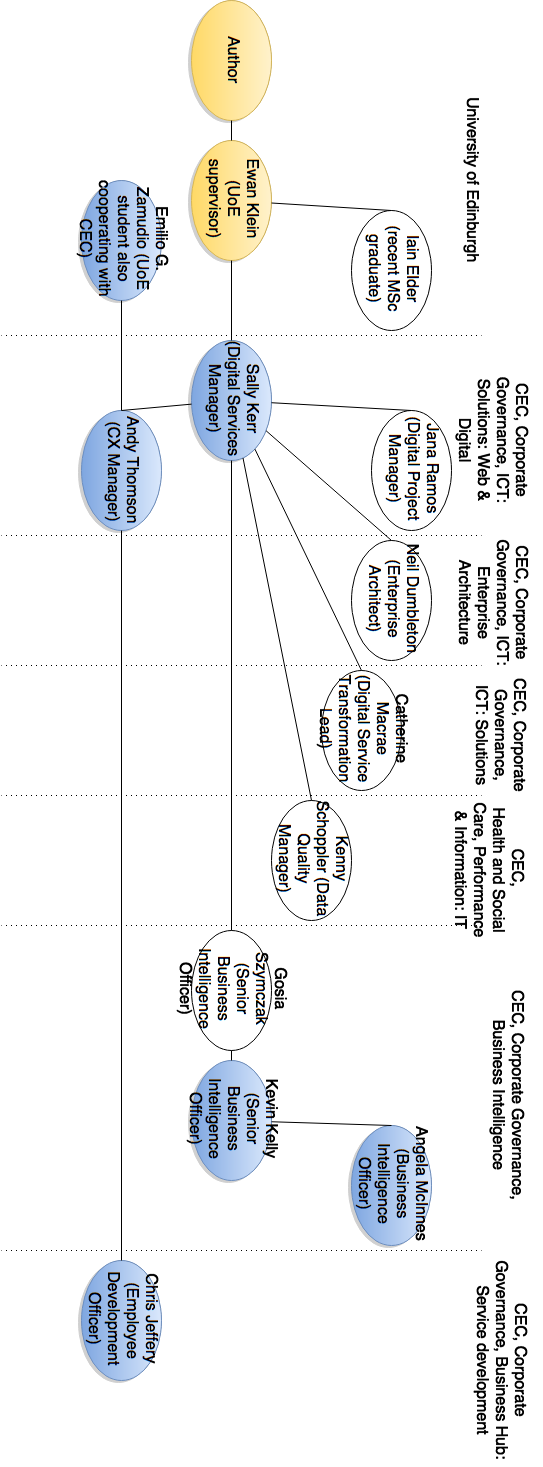
\includegraphics[height=0.95\textheight]{Define_phase_people.png}
  \captionof{figure}{CEC employees involved in the project.}
  \label{normal_case}
\end{center}


At this stage the clients were encouraged to drive the design decisions, e.g. they had a final say in selecting questions to answer with this project. This was mostly done in cooperation with Sally Kerr and Andy Thomson.

The meetings were also trying to select tools that would be used and if possible try to confirm they could be used by building a simple prototype. This was mostly done in collaboration with people from the BI section of CEC, namely Kevin Kelly and Angela McInnes.

Chris Jeffery provided insights about the CRM dataset.

Emilio G. Zamudio was another student of University of Edinburgh that was working on a project with CEC. During discussions with him I wanted to ensure that scopes of our projects do not overlap.
			\subsubsection{First iteration (proof of concept)}
			
The purpose of this stage was to go through the entire cycle of development. Before discussing what kind of analyses would be useful to the Council I had to confirm that it was possible to use the two datasets together and understand what limitations to the process were. There were no existing reports of this kind so I had to create a Cognos package for CRM and Mosaic data.

The Mosaic package has already been imported to the platform as it was being used in other Business Intelligence reports. The process of importing CRM data was manual, but it is planned to be automated in the future. It is assumed that UPRN uniquely identifies the user.

What I needed to do was to add to the Mosaic package on IBM Cognos an external source of data (CRM dataset) using built-in Extract, Transform, Load (ETL) mechanisms, which required administrative access rights. The platform is quite flexible when it comes to file extensions and data formats. Some of the acceptable extensions include: .csv, .xls, .xlsx, .xml. The CRM dataset was extracted from the Council's system and saved as an .xlsx file on a shared network drive. I then created the package and generated a few simple reports as described below.

The above diagram shows the package containing Mosaic and CRM datasets loaded in Cognos. A simple query is then used to show the content of it to verify that it is working as expect - CRM entries are linked with Mosaic entries with UPRN. The results of the query are visualised on the diagram below.

The above screen shot is showing another query which was filtering entries based on the date of creation.

The diagram above shows a chart that was created and here you can see how the layout of the report can be controlled – at the top of the page a list is added.



\begin{center}
  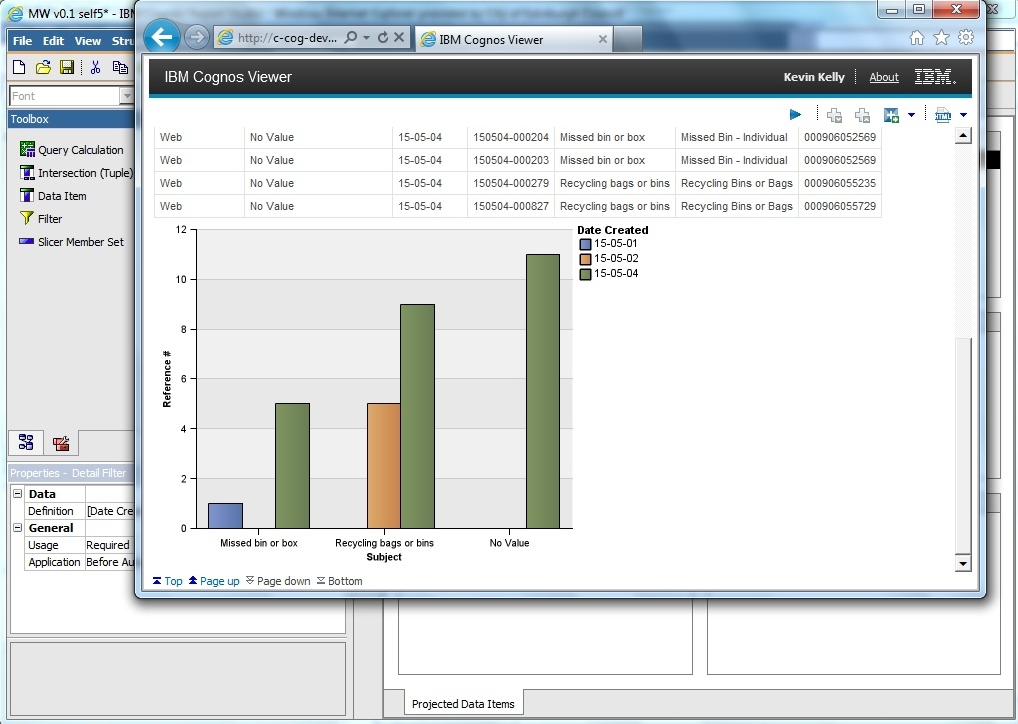
\includegraphics[width=\textwidth]{pre work/2nd day Cognos - processed/creating chart - first chart.jpg}
  \captionof{figure}{first chart}
  \label{normal_case}
\end{center}

In this case, the chart was based on the data from the list above. This was done in order to manually verify that the chart generation happens as expected. Below is the second part of the dataset and the filter used.

\begin{center}
  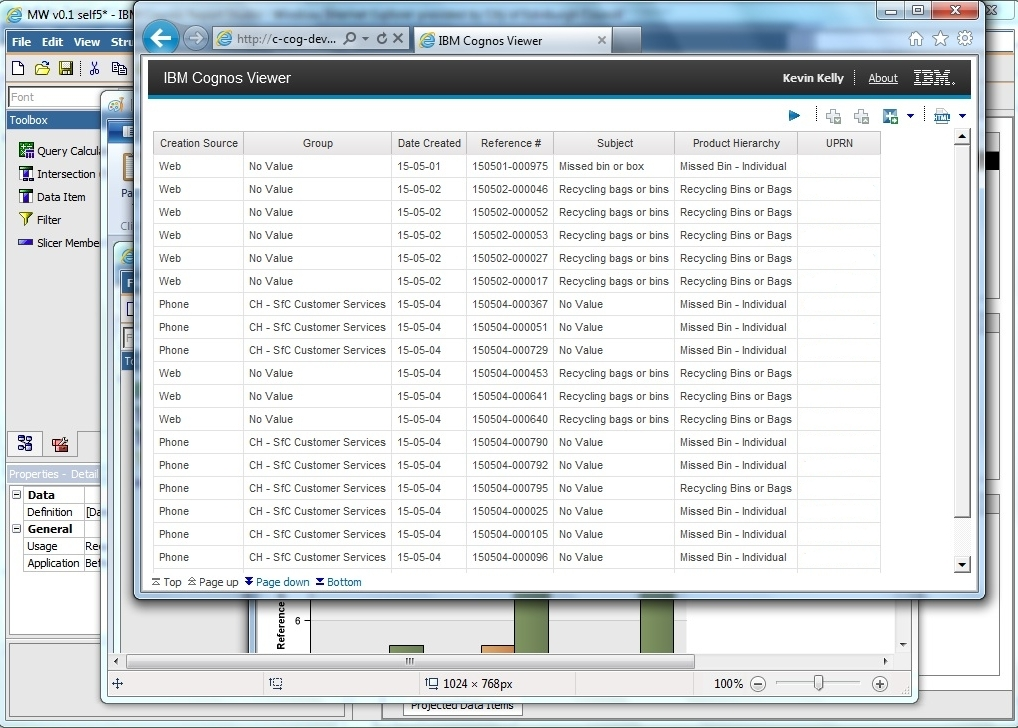
\includegraphics[width=\textwidth]{pre work/2nd day Cognos - processed/creating chart - first chart, data to confirm chart is valid.jpg}
  \captionof{figure}{data to confirm chart is valid}
  \label{normal_case}
\end{center}


\begin{center}
  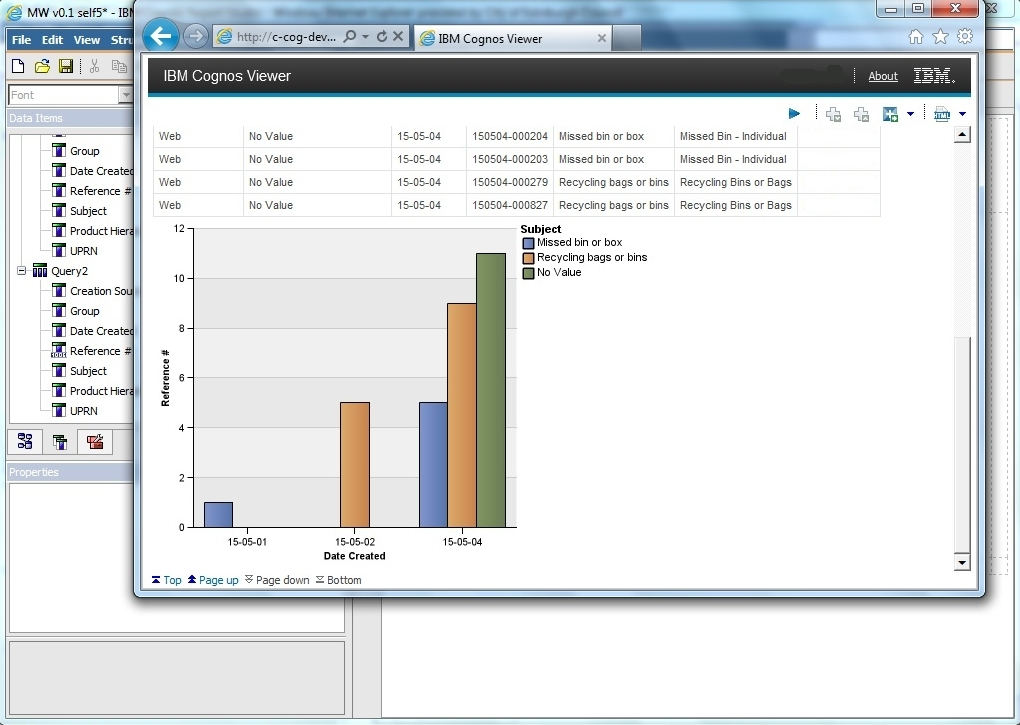
\includegraphics[width=\textwidth]{pre work/2nd day Cognos - processed/creating chart - first chart, other dimension.jpg}
  \captionof{figure}{first chart - other dimension}
  \label{normal_case}
\end{center}


This diagram shows exactly the same dataset, but a different dimension is used for axis x and data series.

Below are a few more examples of reports generated.


\begin{center}
  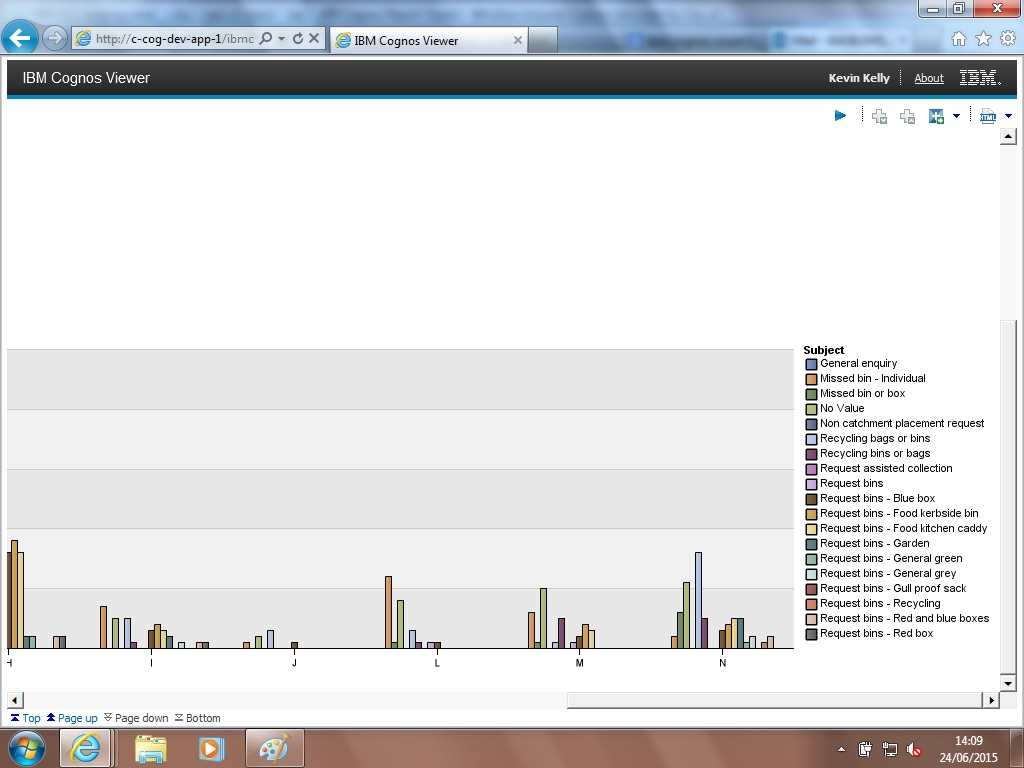
\includegraphics[width=\textwidth]{pre work/2nd day Cognos - processed/second chart, crm and mosaic, all subjects, entire May.jpg}
  \captionof{figure}{second chart – group category, all subjects, entire May, zoom in to legend}
  \label{normal_case}
\end{center}


\begin{center}
  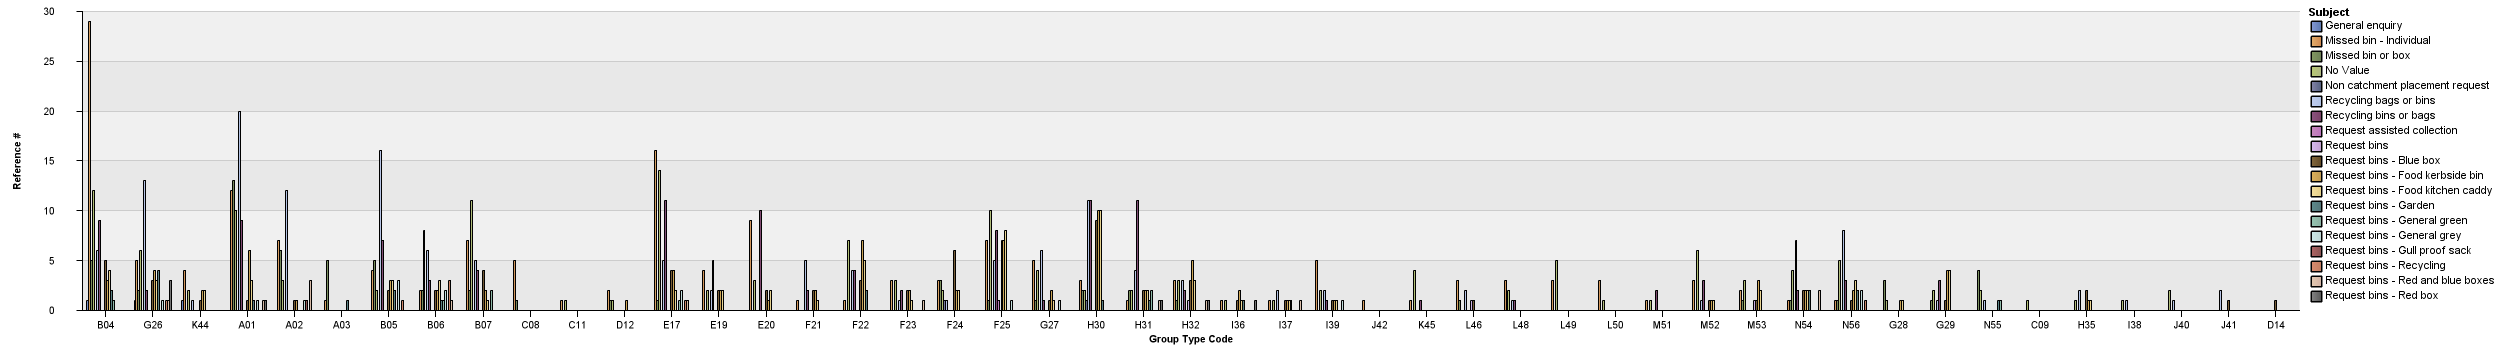
\includegraphics[width=\textwidth]{pre work/2nd day Cognos - processed/group code - all reports.png}
  \captionof{figure}{third chart - group code, all subjects}
  \label{normal_case}
\end{center}



\begin{center}
  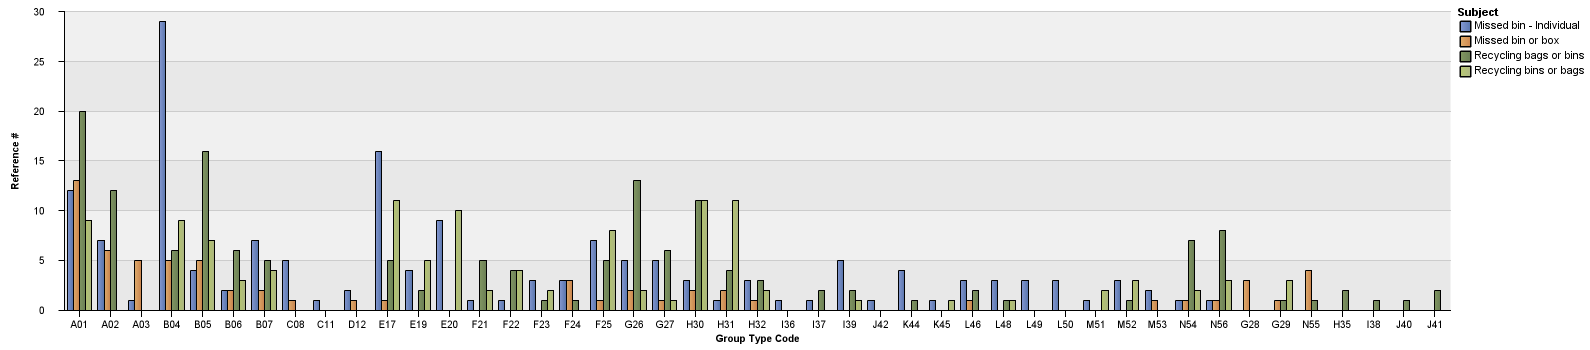
\includegraphics[width=\textwidth]{pre work/2nd day Cognos - processed/group code - bins, recycle.png}
  \captionof{figure}{fourth chart - group code, missed bins, recycling bags (four categories)}
  \label{normal_case}
\end{center}



			\subsubsection{Selected problems}
			
Selected problems experienced in this phase are listed in sections below.			
			
				\paragraph{Linking problem}\mbox{}\\
During the import stage where the CRM data was being added to the Mosaic package there was a problem with linking the two datasets. As a result, I was considering alternative solutions in which I would build the necessary tools.

One of the analysed solutions included setting up a server with an SQL/NoSQL database, populating the database with the CRM and Mosaic data and then conducting analysis using SQL and Python. The focus of the project would shift and the insights generated would be of a different level and quantity. This would decrease usefulness of the project to CEC and move the project away from the initial objective.

After a couple of failed attempts with Cognos I wanted to go through the process step by step and document the problem in as much detail as possible and move on to building the new set up. I was using Cognos documentation in the process \citep{IBM2015, IBM2015c}. Fortunately, the detailed approach adopted has led to finding a solution and the platform could be used in the project.

\begin{center}
  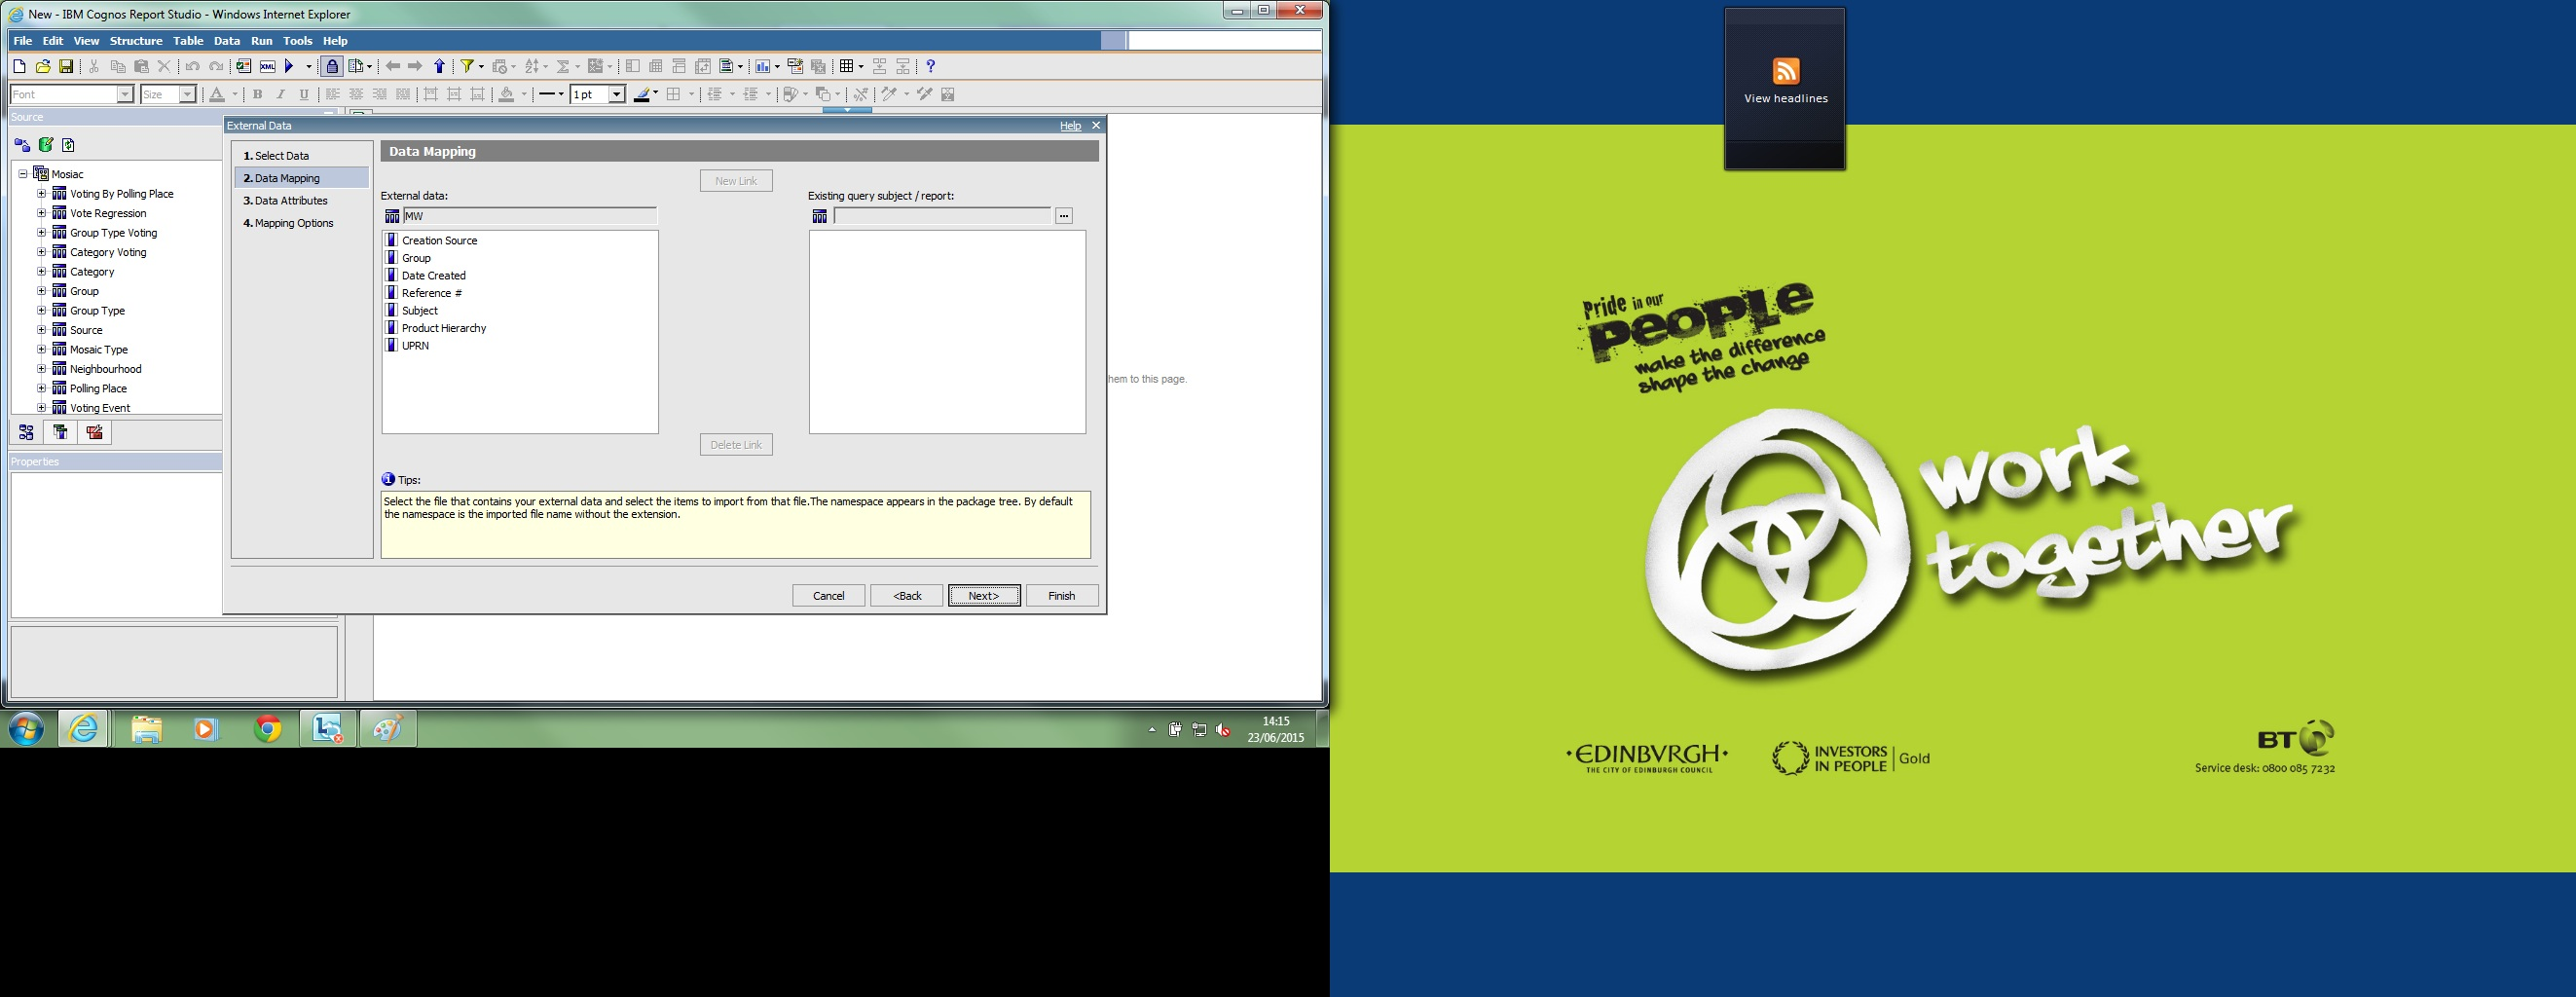
\includegraphics[width=\textwidth]{pre work/1st day Cognos - processed/importing CRM data into Cognos 2.jpg}
  \captionof{figure}{Importing CRM data to Report Studio, CRM data loaded, but Mosaic data unavailable for linking}
  \label{normal_case}
\end{center}
	
				\paragraph{CRM data}\mbox{}\\
One of the problems with analysing CRM data was quality of the data. There are inconsistencies in implementations across different channels. For example, entries regarding requests for recycling bins or bags reported through two different channels had different values in the "subject" field: web - "Recycling bags or bins", phone - "Recycling bins or bags". Initially it was believed that it was an older implementation, but both values were present throughout the entire dataset suggesting both of them were in use. As a result, when analysing the data, filters had to include all possible strings related to the desired value or use a different field – "Product Hierarchy", as was the case with the final reports.

Another problem was related to lack of documentation of the deployment of the CRM system and difficulties in talking to someone knowledgeable about the system. I could not establish in a reliable way the difference between "Product Hierarchy" field and "Subject" field. In the "incidents" table there are entries: "UPRN", "second UPRN", "UPRN 2" but they are not documented anywhere. In cases like this a "best guess" approach had to be used. 
				
		\subsection{Design of the solution}
		
The initial reports served as a learning experience during which I became more familiar with systems and narrowed down the objectives further. I also ensured I would have the necessary access rights before making a decision to pursue this direction.

One of the decisions I had to make regarded data analysis methods. The advantage of using IBM Cognos was a very good integration of many smaller tools (e.g. ETL) and techniques (e.g. changing dimensions of analysis) which made the whole process much more effective and less time consuming. Consequently, I would be able to conduct much more analyses that would present more value to the Council.

Selected advantages of using IBM Cognos:
\begin{itemize}
\item can be easily accessed by CEC employees (e.g. in their web browser)
\item can be used by CEC employees in the future (they can feed my reports with other data extracts and conduct the same analysis on it)
\item can be used as a starting point for future reports (they can go through my files to see how I did it, they can expand them adding or rearranging some parts of it)
\item it is in line with the strategic direction of development of the Council so I would be directly contributing to the efforts of the Council
\item it is within the CEC environment (no need to migrate my solution to CEC environment)
\end{itemize}

In terms of ideas for analysis, I developed a list of questions I thought were relevant from the perspective of someone implementing or improving transactions at the Council. I than discussed it with CEC employees (Sally Kerr and Andy Thompson), added their ideas and gave them the final word about which ones to implement. The result was a list of three questions and a decision regarding further direction.
		
		\subsection{Design brief for the next stage}
		
The data analysis will be conducted using IBM Cognos platform and it will use Mosaic Experian package combined with an extract of the data from the CRM system. The reports generated will not be of performance indicators nature, but will try to find data that can show behaviour of citizens manifesting in the data. They are not (primarily) intended as monitoring tools, but rather as ways of expanding perception of what is happening in service delivery. The three main questions that will be answered are listed below and they are described in detail in the following sections:
\begin{enumerate}
\item Cases of intentional use of multiple channels for the same issue
\item Patterns of behaviour across different channels
\item Who are the primary users of CEC services
\end{enumerate}
		
			\subsubsection{Report 1 - cases of intentional use of multiple channels for the same issue}
			
This analysis is aiming at identifying cases where citizens want to report an issue, but do not trust in it being handled the same way through different channels. The reasoning behind such behaviour is that if many tickets are opened for the same problem, one of them will "get the job done". It will be solved the quickest possible way, because if the process behind one channel has more resources available it will be handled quicker than with the process behind another channel.

The underlying assumption is that entries in the CRM system will not be identified as related to the same problem and that time of delivery differs across different channels.

The purpose of this analysis is not to provide evidence about the assumptions being right or wrong, but to verify if such behaviour exists among receivers of the Council services.
			
			\subsubsection{Report 2 - patterns of behaviour across different channels}
			
The purpose of this analysis is to understand patterns of behaviour of citizens across many channels.

Some of the patterns that might be revealed include:
\begin{itemize}
\item The user initiated a service through a channel of preferred choice (e.g. web-form). However, after not hearing from the Council for some time, the user is unsure about the status of the process and uses a channel that is considered trustworthy (e.g. face-to-face) to confirm its state.
\item If the above pattern occurs only for one type of transaction it might suggest a problem with a particular service. For example, if many users try to report a missed bin over a web-form, but eventually use a phone to do it (or switch after a few uses) it might highlight issues with this particular web-form.
\item An active user who uses a particular service is trying out a digital interface, but for some reason goes back to how he access it before
\item Numerical evidence for how quickly people adapt new channels (e.g. how effective an information campaign was)
\end{itemize}	
			
			\subsubsection{Report 3 - who are the primary users of CEC services}
			
Designing is a task that should be conducted with the user in mind and having an understanding of who is the primary receiver of the design helps tremendously. For this reason, designers use "personas" which make it easier to model how the user thinks or behaves. The more detailed and accurate information about the user one has, the  better design decisions one can make, which results in interfaces and services that better fit the needs of people.

The questions that will be answered within this part of work are trying to increase the understanding of users receiving Council's services. In particular, three user groups are recognised:
\begin{itemize}
\item never used CEC services
\item uses CEC services occasionally (defined here as having no more than three interactions with CEC)
\item active user of CEC services (more than three interactions with CEC)
\end{itemize}

The analysis is trying to identify socio-economic backgrounds that users from all three groups have. Because CRM data contains only data about citizens who used CEC services it will not contain information about the first group. However, by determining who is interacting with CEC one can conclude who is not using those services. In other words, social groups that do not appear in the CRM dataset can be categorized into the first group.

Some of the questions that could be answered include:
\begin{itemize}
\item who are primary users in general
\item which social group has the most interactions within a service
\item which service is most popular within a social group
\end{itemize}

	\section{Develop}
	
The implementation stage of the project started with three objectives coming from the previous phase. Subsequently, three reports were generated to provide analysis in those areas.

Development started in a fresh environment. CEC provided me with a designated work space together with a laptop and all the access rights necessary for the implementation (access from the preliminary stage was revised and a different setup was used). Due to this, the IBM Cognos package containing Mosaic Experian and CRM data had to be recreated from scratch as described in the Define phase.

The process in all three cases was to design a technical solution first and then implement it. The solution, a generated report, would consist of a number of queries that would provide results necessary to answer a question or an intermediate step (in more complex cases) that lead to the desired insights. For more information on stages in the report creation, please see Appendix A containing a list of files used in the process.
	
		\subsection{Report 1 - cases of intentional use of multiple channels for the same issue}
		
This report is trying to provide evidence for existence of a specific type of behaviour where citizens report one and the same issue using many channels at the same time.

Proving such behaviour using solely data analysis is very difficult and should not be left only to an algorithm. One of the problems with this kind of analysis is that behaviour of people with different intents might manifest in the data in the exactly same way. The report might group in the same category users with "scattershot" approach, but also non individual users like landlords, who visit many sites and then report a bulk of issues, residents who struggled with submitting a web-form or first time users of CEC services who were helped in submitting a web-form by a consultant over the phone.

It has to be stressed that this analysis is not trying to automatically mark people as "bad users", but instead bring attention of a service manager to cases of unusual uses of the system. They might be pointing to a number of issues such as different delivery times across different channels, lack of trust in digital channels, low effectiveness of a channel in addressing a user need. They should be analysed and investigated further and should be treated as potential inspirations or initial influences for further improvement of service delivery.

			\subsubsection{Technical design}
Query 1: gather all relevant data (do not include entries if channel is not specified) and add a counter for how many issues someone filed on one day\\
Query 2: filter results of Query 1 so that only people who reported more than one issue on one day regarding the same subject are left\\
Query 3: filter out from Query 2 cases with only one occurrence of such behaviour (of multiple issues regarding one subject reported on the same day)

			\subsubsection{Implementation}

\begin{center}
  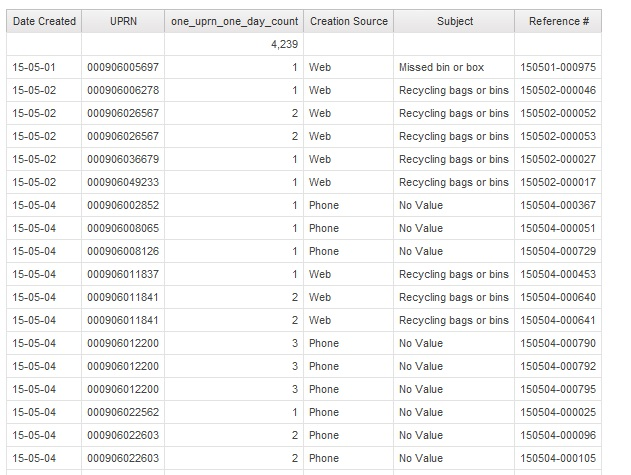
\includegraphics[width=\textwidth]{Report 1/report 1, query 1.jpg}
  \captionof{figure}{Report 1, Query 1}
  \label{normal_case}
\end{center}

\begin{center}
  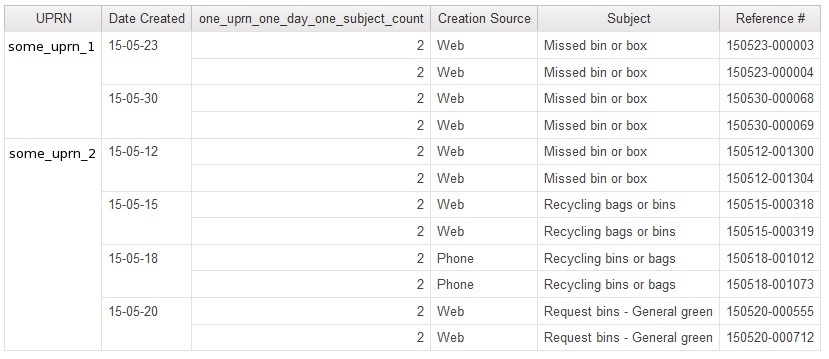
\includegraphics[width=\textwidth]{MW 12.08/MW 12.08/Report 1, query 3.jpg}
  \captionof{figure}{Report 1, Query 3}
  \label{normal_case}
\end{center}
	
			\subsubsection{Additional work}
			
There were only two cases found of multiple cases of reporting a few times a day and none of them was unwanted behaviour. It can be speculated that those were situations in which someone was having problems using CEC interfaces (cases of double entries with very short time distance).

Query 4 was created after conducting the above analysis. Its purpose was to provide a general overview on the number of multiple reports to give an idea of how much people struggle with an interface and how quickly they learn it.

Query 4: count number of occurrence of such behaviour (how many times did someone report the same issue more than once on the same day)

\begin{center}
  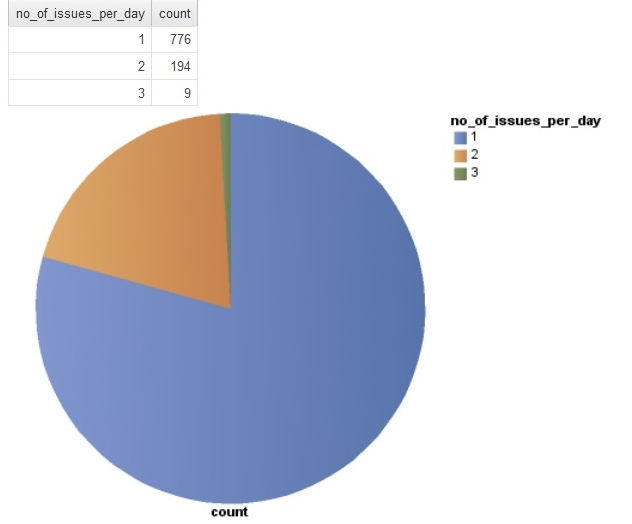
\includegraphics[width=\textwidth]{MW 12.08/MW 12.08/Report 1, query 4, cut.jpg}
  \captionof{figure}{Report 1, Query 4}
  \label{normal_case}
\end{center}



In simple words, there were 194 people in May 2015 who on two separate occasions reported on the same subject, on the same day.
			
		\subsection{Report 2 - patterns of behaviour across different channels}
		
This part of analysis is trying to cast some light on behaviour of citizens across different channels.

It is based on two counters. The first one provides information about the total number of issues reported by a citizen ("count no of issues"). The second one counts the number of separate channels used to report those issues ("channels used"). Then filters are used to remove from the report cases with the number of issues below two ("count no of issues \textgreater 1") and the number of channels used below two ("channels used \textgreater 1").

In order to make the results easier to analyse, entries are grouped using UPRN – entries coming from one user are listed next to each other. Within this group, they are ordered using reference number ("Reference \#"). The reference number is used instead of date of creation because there are multiple cases where there is more than one entry during a day. In those situations, ordering by the date does not ensure the same sequence as the sequence of creation. A reference number on the other hand, consists of two parts: the day of creation and a serial number assigned in an ascending manner and thus the original sequence can be deduced. In the following example, both reference numbers were created on the same day, but the second one was created later which can be determined by the second part of the string:
\begin{lstlisting}
150511-000837
150511-000849
\end{lstlisting}

The diagram below presents part of the report that was generated.

Citizen with UPRN 000906026074 submitted a "Missed bin or box" request through the web-form on fifth May and made a phone call the next day regarding a service from the same "Product Hierarchy". It can be speculated, that both interactions were about the same issue. In order to verify such claim these interactions would have to be investigated further, e.g. using comments left by consultants (unstructured data) \citep{baars2008management}. Such additional information would be extremely useful in determining reasons for the user following up over the phone.

Citizen with UPRN 000906037096 submitted two queries for the same issue on 12th of May. The next day he submitted again two queries over the web for a different service, but what is really interesting is that after submitting them he made a phone call to the Council. This is a great example of identifying a situation where someone started with the web-form, but then for some reason made a phone call anyway. It might have been a simple question about the form, but clearly the person made the call after going through the web-form. It might be the case that putting the information the user requested on the form would help other users in the future.
		
			\subsubsection{Technical design}
			
Query 1: count number of issues reported by a citizen, count number of channels used to report those issues, filter out number of issues below two, filter out number of channels used below two
			
			\subsubsection{Implementation}

\begin{figure}[hp]
\centering
     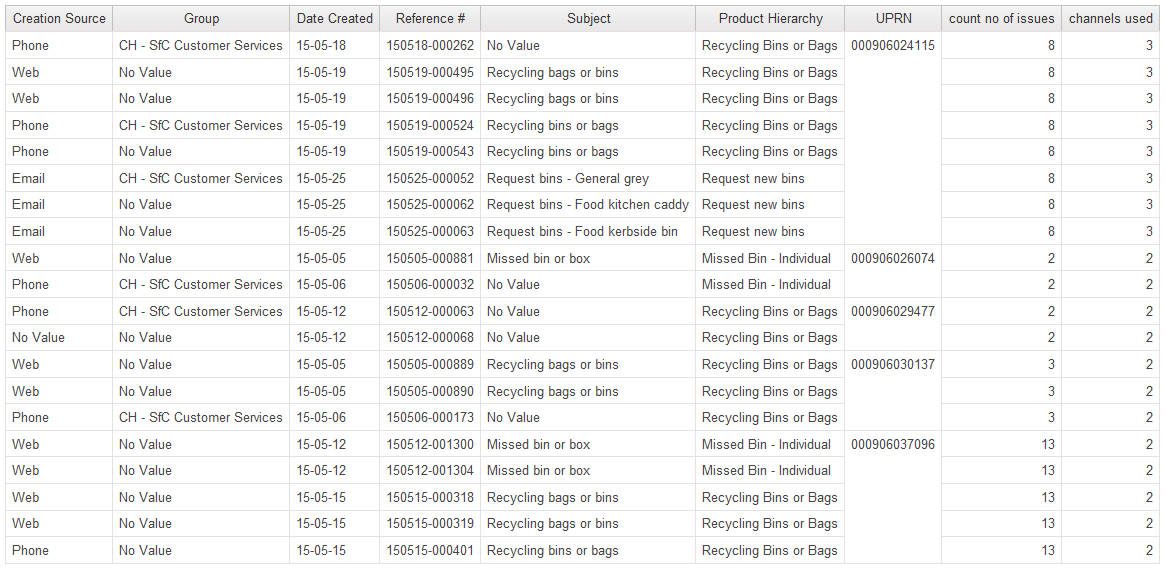
\includegraphics[width=\textwidth]{Report 2/report 2.2 page 2.png}
      \caption{Report 2, example}
       \label{normal_case}
\end{figure}
			
		\subsection{Report 3 - who are the primary users of CEC services}
		
This analysis starts from identifying users belonging to two categories as described in the Define phase, i.e. citizens who interacted up to three times with the Council and active users with more than three issues reported. After that, a series of queries are used in order to provide insights about socio-economic background of users.

The letters at the bottom of charts (A,B,C,…) are Mosaic groups. Detailed information about each group can be access using Mosaic Portal – Segmentation. There, information is interpreted and visualised in a more human friendly way, as described in the Discover phase.

			\subsubsection{Technical design}
			
Query 1: gather relevant data, count number of all interactions of a user, assign a value based on the counter identifying the category as described above (up to three, above three), assign Mosaic groups to entries\\
Query 2: Which services are the most popular among people in both categories? – generate a chart with services on axis x, number of entries on axis y (counted by "Reference \#" field, count total aggregation) and data series for up to and below the threshold level\\
Query 3: Which Mosaic groups do people from both categories belong too? (which social groups use CEC services most actively) – generate a chart with Mosaic groups on axis x, number of entries on axis y (counted by "Reference \#" field, count total aggregation)\\
Query 4: Which services are being used by different Mosaic groups? – generate a chart with Mosaic groups on axis x, number of entries on axis y (counted by "Reference \#" field, count total aggregation) and data series for different services\\
Query 5: Which Mosaic group is the most active within a service? This part of the report is using "value prompts" which allow to select a service which will be analysed. It shows a chart for the selected service.
			
			\subsubsection{Implementation}
			
			
\begin{center}
  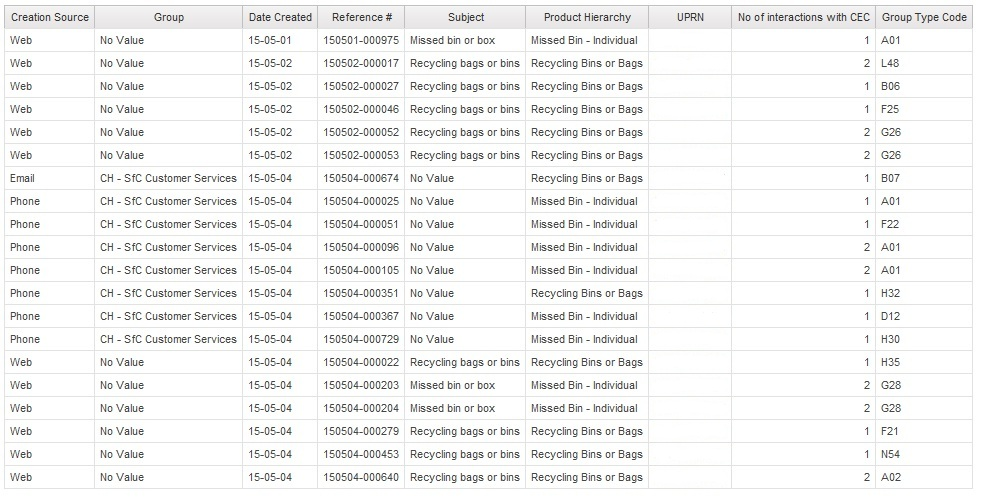
\includegraphics[width=\textwidth]{Report 3/list of citizens who had at most 3 interactions with the Council in May.jpg}
  \captionof{figure}{Report 3, Query 1 (up to three interactions)}
  \label{normal_case}
\end{center}
			

\begin{center}
  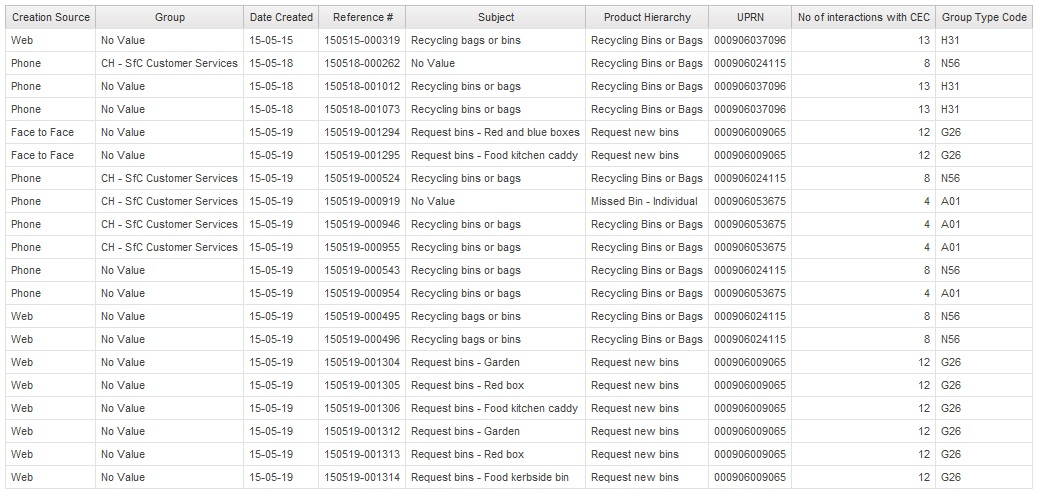
\includegraphics[width=\textwidth]{Report 3/list of citizens who had more than 3 interactions with the Council in May.jpg}
  \captionof{figure}{Report 3, Query 1 (above three interactions)}
  \label{normal_case}
\end{center}



\begin{center}
  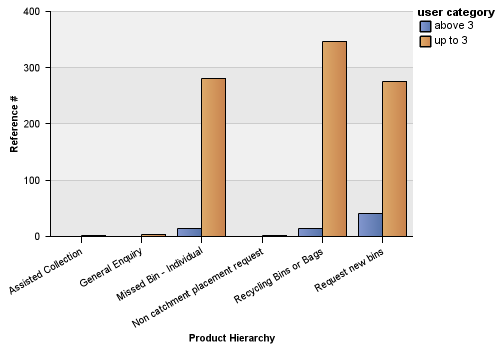
\includegraphics[width=\textwidth]{MW 12.08/MW 12.08/Report 3, query 2, axis sorted.png}
  \captionof{figure}{Report 3, Query 2}
  \label{normal_case}
\end{center}


\begin{center}
  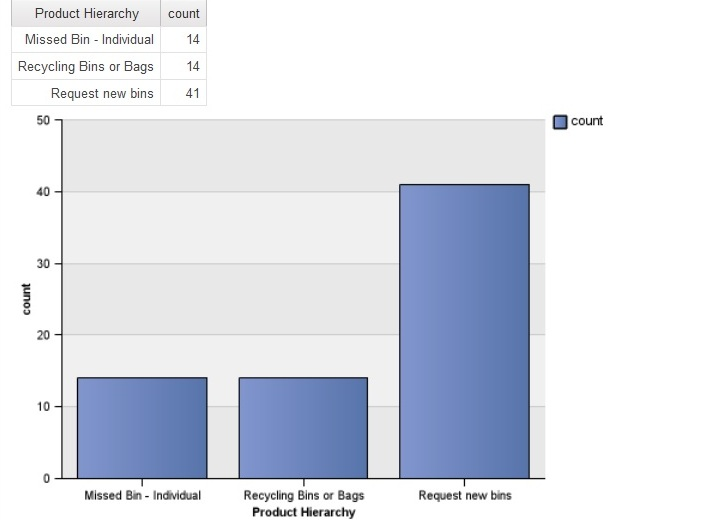
\includegraphics[width=\textwidth]{Report 3/report 3, 1.1.jpg}
  \captionof{figure}{Report 3, Query 2 (above three)}
  \label{normal_case}
\end{center}



\begin{center}
  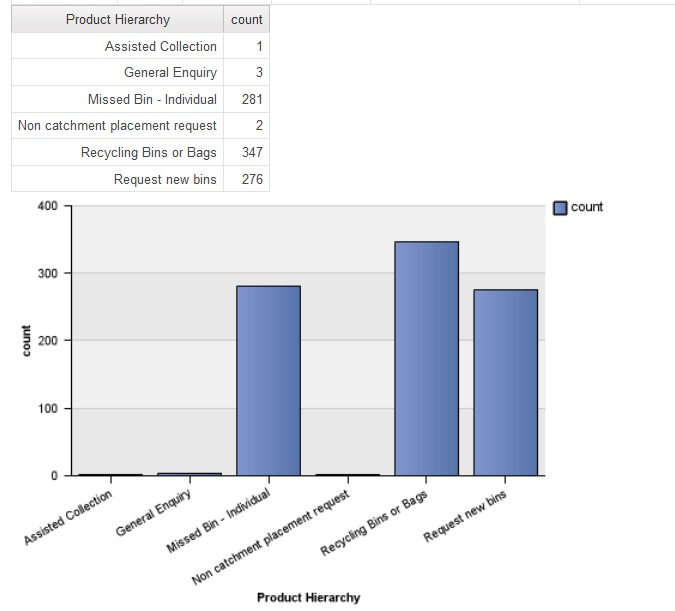
\includegraphics[width=\textwidth]{Report 3/report 3, 1.2.jpg}
  \captionof{figure}{Report 3, Query 2 (up to three)}
  \label{normal_case}
\end{center}


\begin{center}
  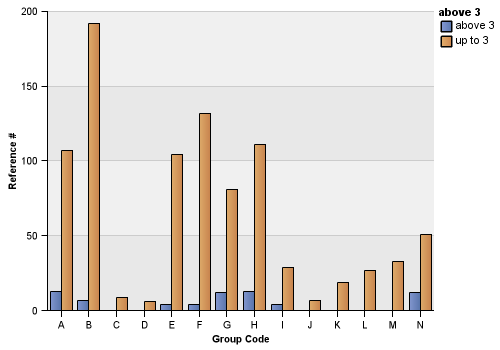
\includegraphics[width=\textwidth]{Report 3/report 3, 3.2 both on one chart.png}
  \captionof{figure}{Report 3, Query 3}
  \label{normal_case}
\end{center}


\begin{center}
  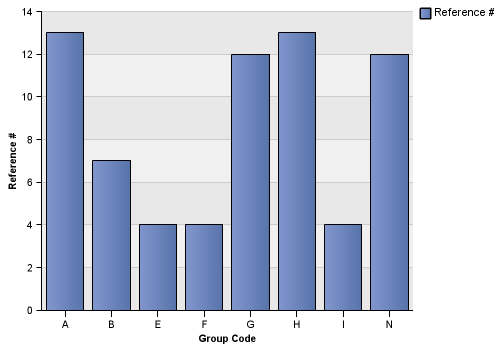
\includegraphics[width=\textwidth]{Report 3/report 3, 3.1 above 3.png}
  \captionof{figure}{Report 3, Query 3 (above three)}
  \label{normal_case}
\end{center}


\begin{center}
  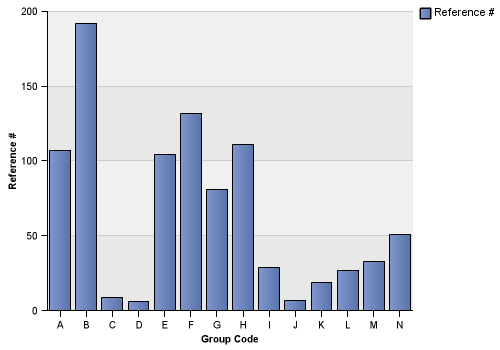
\includegraphics[width=\textwidth]{Report 3/report 3, 3.1 up to 3.png}
  \captionof{figure}{Report 3, Query 3 (up to three)}
  \label{normal_case}
\end{center}


\begin{center}
  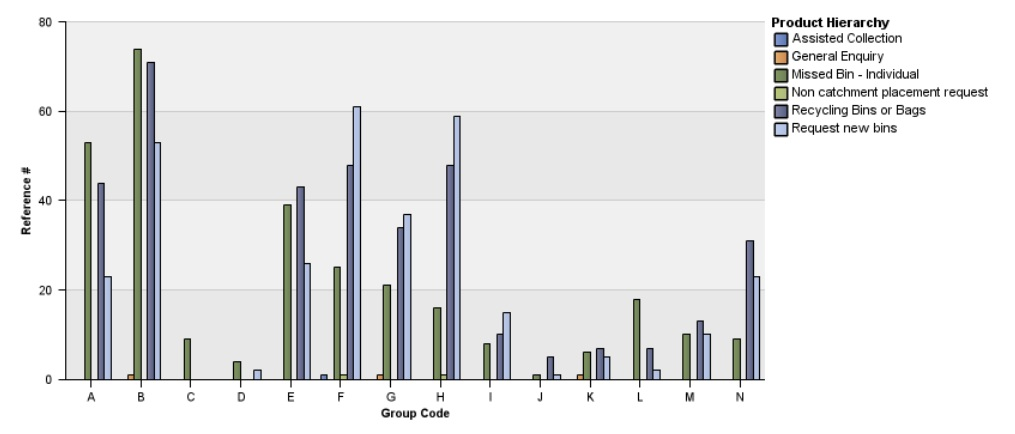
\includegraphics[width=\textwidth]{Report 3/report 3, 2.1.jpg}
  \captionof{figure}{Report 3, Query 4}
  \label{normal_case}
\end{center}

\begin{center}
  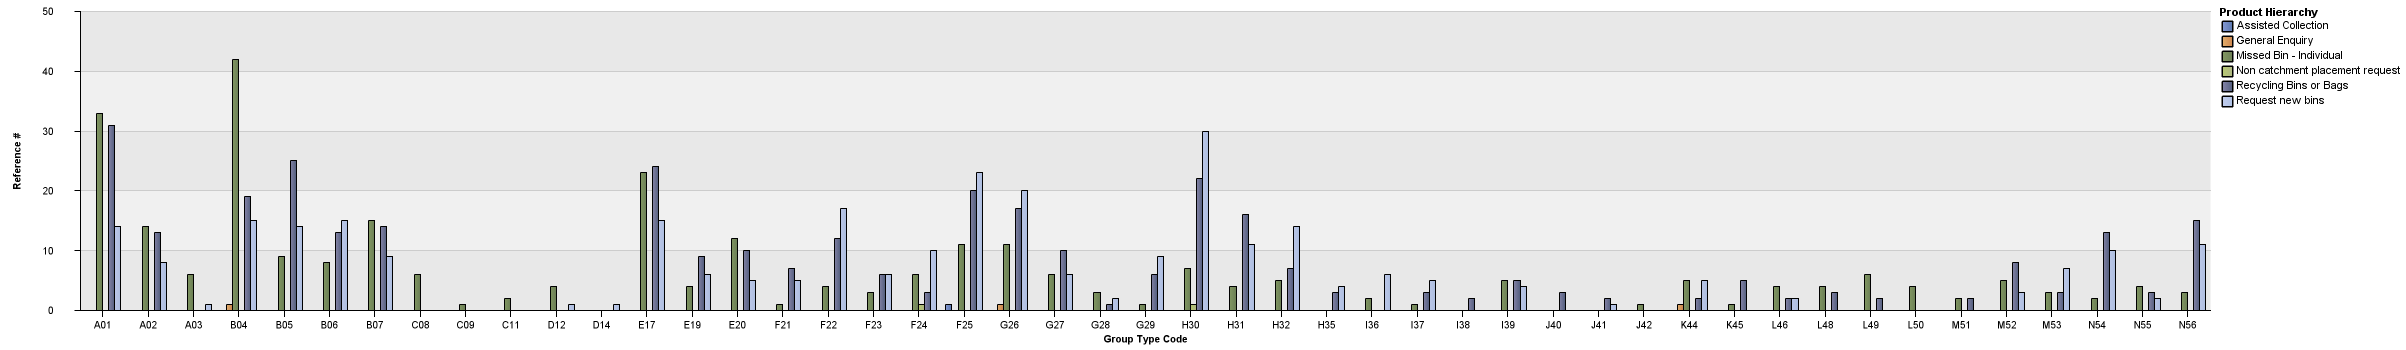
\includegraphics[width=\textwidth]{Report 3/report 3, 2.2.png}
  \captionof{figure}{Report 3, Query 4 (more granular user groups - Mosaic group and type)}
  \label{normal_case}
\end{center}

\begin{center}
  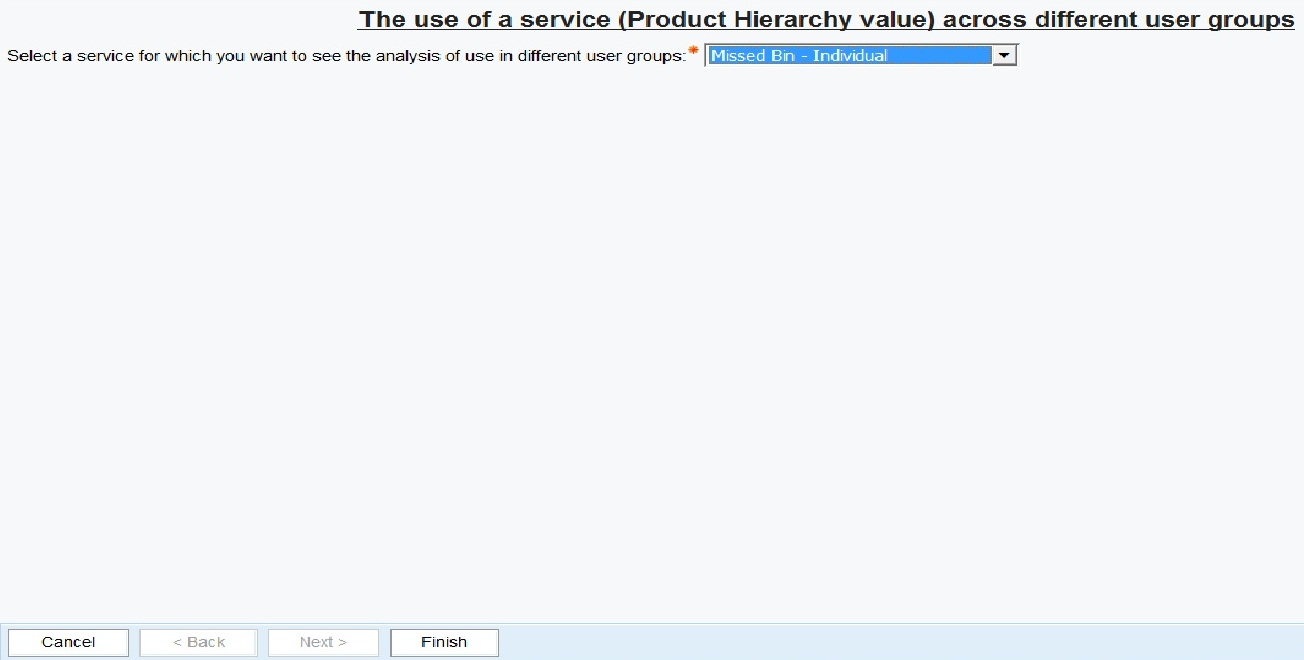
\includegraphics[width=\textwidth]{Report 3/report 3, 2.3 select screen, selected value.jpg}
  \captionof{figure}{Report 3, Query 5. Value prompt page with selected service - "Missed Bin - Individual"}
  \label{normal_case}
\end{center}


\begin{center}
  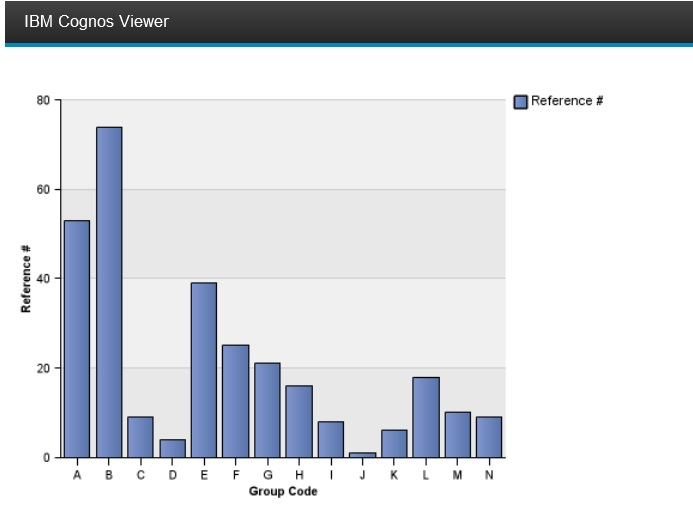
\includegraphics[width=\textwidth]{Report 3/report 3, 2.3 group code chart.jpg}
  \captionof{figure}{Report 3, Query 5}
  \label{normal_case}
\end{center}


\begin{center}
  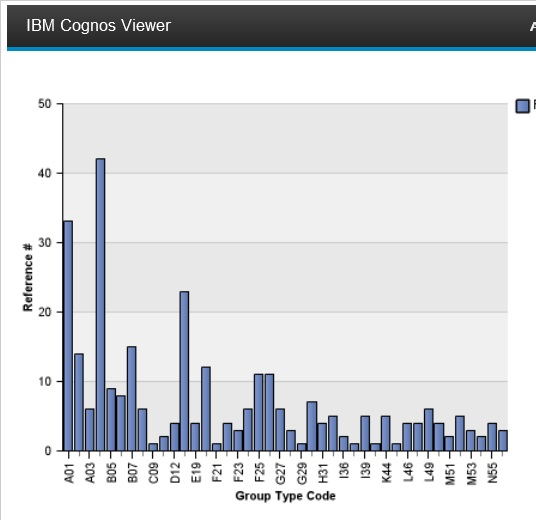
\includegraphics[width=\textwidth]{Report 3/report 3, 2.3 group type code chart.jpg}
  \captionof{figure}{Report 3, Query 5. (more granular user groups - Mosaic group and type)}
  \label{normal_case}
\end{center}


	\section{Deliver}
	
		\subsection{Presentation at the Council}
		
In the delivery phase, I gave a presentation to CEC employees. The purpose was to present the project as a whole, show how to use the reports and evaluate their usefulness (receive feedback). Below are some quotes from the meeting in which Sally Kerr, Andy Thomson and Gosia Szymczak took part.\\\\
''It's very useful for us as well to have somebody coming from outside and giving us a fresh perspective and it is work that we have to continue with, so it's really interesting''\\
Sally Kerr\\\\
''One of the questions that we had, which obviously I think you didn't really have time to completely develop or it might be in your dissertation, was looking at (…) number of profiles we had and try to look at usage across those, because when we had originally done those profiles we made a best guess at the forms they would use the most. One of the questions was, did we get it right? (…) it would be very interesting to do that, because I think we are at a stage, moving with the new ICT supplier, to review that, to actually look at that model and then how is the supply going forward and also in terms of the communication campaign as well''\\
Sally Kerr\\\\
''We haven't been doing anything as in depth as that because nobody has asked us to do that. It's interesting just to see (…) the person is trying and trying to do it three times on the web and it's not going anywhere so there must be something.''\\
Gosia Szymczak\\\\
''I think the problem that we have (…) there is a bit of assumption with analysis there, which is very difficult to get away from unless you have user tests face-to-face (…) which I would recommend that we do, because however much (…) tracking tools, I still think you need to be going back to citizens just to actually make sure you are developing in the best way.''\\
Sally Kerr\\\\
''This is very interesting, just to get the indicators is very interesting and it's something we can share, it's just really important.''\\
Sally Kerr\\\\
''If a person is recording two or three times the same thing does that mean it's one complain or is it three complaints from the same person. It's helping us understand and analyse the stats, have a look at the stats, if the stats are correct, because there are three complaints from the same person on the same thing from the same address.''\\
Gosia Szymczak\\\\
''What we need is a good methodology for how you would do that (solve problems experienced by users), because we don't have the resource to give that kind one-to-one all the time (go through an individual problem), so this is really useful.''\\
Sally Kerr\\\\
''To be honest, we should be really carrying out this kind of analysis regularly to actually see if behaviours are changing. (…) That's a recommendation I would make, that we should be looking at how we do that for the future.''\\
Sally Kerr\\\\
''From University's point of view there are definitely opportunities, now we know how it all works for students to be involved with a particular piece of work if it's felt to be of interest. Working with BI on that, we will discover other areas that will be very useful as well.''\\
Sally Kerr\\

	\section{Problems}
	
In this part, selected problems experienced during the project are described. They are listed here in order to document the process as well as provide feedback for the design process:
\begin{itemize}
\item Due to informal form of the cooperation, for a substantial part of the project, I did not have a pass to the building. It would be useful to have a starting date fixed in order to prepare a temporary pass and access rights for systems.
\item The fact that the project had an open nature at the beginning was a very important part of it and helped in achieving a natural convergence between different teams of CEC and making the outcomes relevant and useful to the Council. However, this should not result in not having a clear business owner (e.g. Business Intelligence and Digital Service). Allocating even a small amount of resources (time of people involved) by senior management would help the project by not putting the burden of excessive time on CEC employees and would help in getting access to the licensed platforms within existing structures.
\item In order to work with ICT systems in the Council a workstation (from the Council) is required. It would help to use a laptop together with the account created for the temporary pass that would have all the necessary accesses. During the project, the use of a laptop had to be supervised (putting additional burden on CEC employees) together with an account that had extremely limited storage space.
\item Difficulties were experienced when creating charts using calculated fields (no problems using values from a database). Charts do not work with automated aggregation function, you have to use "none" as the aggregation function.
\begin{center}
  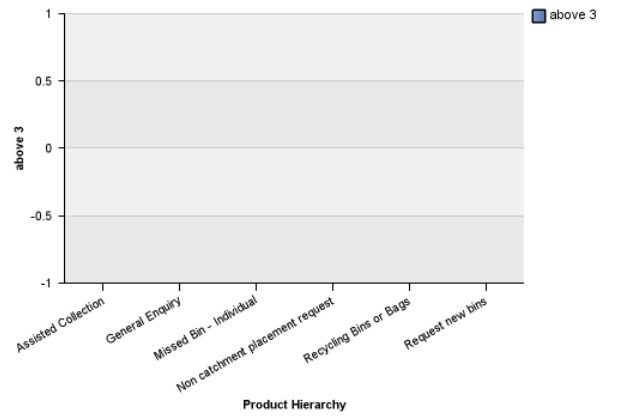
\includegraphics[width=\textwidth]{Report 3/report 3, chart 1, aggregation function not set.jpg}
  \captionof{figure}{Report 3, Query 2. Aggregation function not set to "none"}
  \label{normal_case}
\end{center}
\item The CRM data source file had blank entries. IBM Cognos considered them valid (did not filter them out). They were showing up in all analyses as empty and could not be filtered out. There was about 4200 of them. They were removed from the extract manually.
\begin{center}
  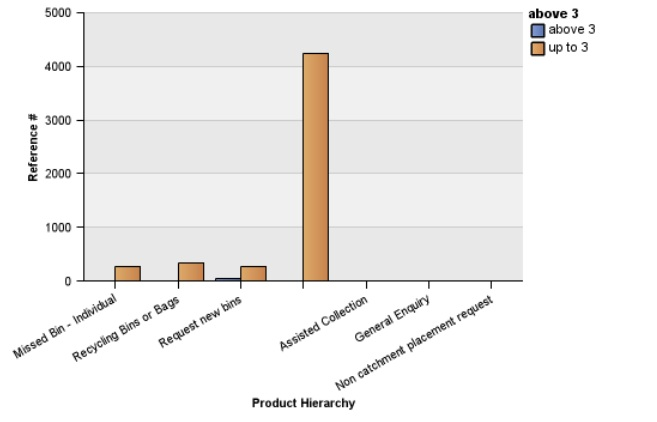
\includegraphics[width=\textwidth]{Report 3/data_source_problem.jpg}
  \captionof{figure}{Report 3, Query 2. Empty entries showing up in all analyses}
  \label{normal_case}
\end{center}
\item When a filter was implemented and then removed a result would be generated (different from when the filter was present). However, if the platform was restarted the results were different (for the same report).
\begin{center}
  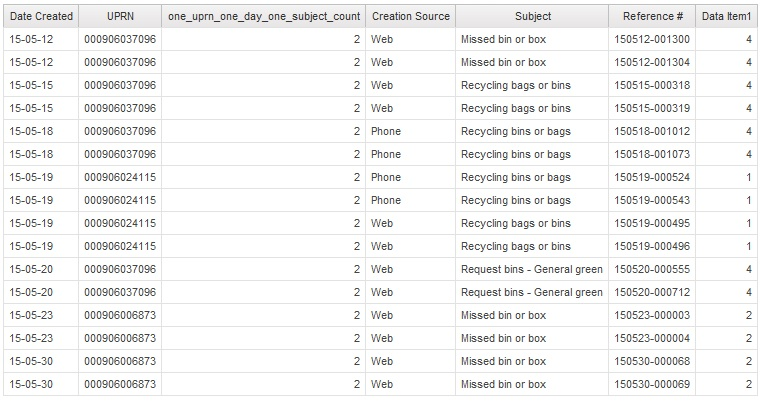
\includegraphics[width=\textwidth]{Report 1/problem.jpg}
  \captionof{figure}{before restarting platform}
  \label{normal_case}
\end{center}
\begin{center}
  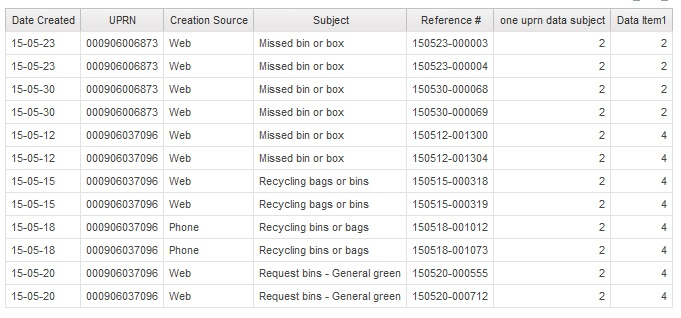
\includegraphics[width=\textwidth]{Report 1/report 1, query 3.jpg}
  \captionof{figure}{after restarting platform}
  \label{normal_case}
\end{center}

\end{itemize}

